\chapter{Sprint 4}
\label{chap:S5}

In the fourth sprint, the 8th and 9th week of the project, the system design is finalized. It was the period when the whoe group was working confidently with implementation and report writing. We had already started modifying the system in the previous sprint, and the whole group knew what tasks they had been assigned. The goal of the sprint was to complete the system with all modifications we had decided upon during the previous sprint, and completing as much of the report as possible.

\section{Sprint plan}
\label{sec:S5Plan}

The plan was fairly clear this sprint. Tasks were given a priority and a time estimate. Tasks with a priority of Major had to be completed as soon as possible, then tasks with Normal priority, and finally Low priority tasks if time permitted. Event registration was the system this sprint would focus the most on, as well as a redesign of the front page based on the suggestions given at the presentation in Oslo during sprint 3.

\paragraph{} As part of the plan for a new design, we would start looking into the Google design guidelines for web pages, especially looking for tips on color changes. Other plans included implementing sharing to other social media, designing logos for each interest. We also spent some time discussing the domain name for the site, and would advise the customers in setting up the site.

\section{Duration and workload}
\label{sec:S5Duration}

\begin{minipage}{\linewidth}
\centering
\setlength{\tabcolsep}{22pt}
\textbf{Sprint 4:} 
\smallskip
\rowcolors{1}{blue!20}{blue!10}
\begin{tabular}{ |l l| }
	\hline
	\it{Duration} & 2 weeks \\
	\it{Start} & October 20th. \\
	\it{End} & November 2nd. \\
	\it{Workload} & Hours spent by the entire group on Sprint 4. \\
	\it{Goal} & 20-25 hours per person \\
	\hline
\end{tabular}
\end{minipage}\\%
%
\begin{minipage}{\linewidth}
\setlength{\tabcolsep}{15pt}
\centering
\rowcolors{1}{blue!20}{blue!10}
\begin{tabular}{ |l|l| }
	\hline
	\multicolumn{2}{|c|}{\cellcolor{gray!25} Workload} \\
	\hline
	\it{Planning} & 25 hrs\\
	\it{Development} & 58 hrs\\
	\it{Design} & 20 hrs\\
	\it{Documentation} & 83 hrs\\
	\it{Testing} & 10.5 hrs\\
	\hline
	\textbf{\textit{Total Workload}} & 196.5 hrs\\
	\hline
\end{tabular}
%Caption here
\captionof{table}{Workload of Sprint 4. \label{tab:S4Workload}} 
\end{minipage}

The group's amount of work went down compared to the previous sprint. Some people were away, and ill. It is further discussed in \ref{sec:S5RetrospectiveDynamics}.

\section{Sprint backlog}
\label{sec:S5Backlog}

\begin{minipage}{\linewidth}
\setlength{\tabcolsep}{12pt}
\centering
\rowcolors{1}{blue!20}{blue!10}
\begin{tabular}{|p{1cm}|p{4cm}|p{2cm}|p{2cm}|}
\hline
\cellcolor{gray!25} ID & \cellcolor{gray!25} Description & \cellcolor{gray!25} Estimated Time & \cellcolor{gray!25} Actual Time \\
\hline
CDP-25 & \it{Design of home page} & 2d & 2d2h \\
CDP-13 & \it{Navigation between pages} & 4h & 4h \\
CDP-8 & \it{Event creation} & 3d & 3d4h30m \\
CDP-21 & \it{Photos should display more details (when was the photo uploaded, by whom)} & 4h & 4h \\ 
CDP-36 & \it{Photo rating} & 12 hrs & 1d \\
D4.1 & \it{Icons fo the different interests} & 3hrs & 4hrs \\
RPT-41 & \it{Finish Sprint 1 for the report} & 3hrs & 3hrs \\
RPT-42 & \it{Sprint 2} & 18h & 1d2h \\
RPT-43 & \it{Sprint 3} & 12h & 12h \\
RPT-47 & \it{Introduction} & 3h & 3h \\
RPT-71 & \it{Risk management} & 1d & 1d2h \\
RPT-72 & \it{Quality Assurance} & 5h & 5h \\
RPT-29 & \it{Restructuring/finishing preliminary studies} & 6h & 5h \\
R4.1 & \it{Proofreading} & 5h & 5h \\
\hline
\end{tabular}
\captionof{table}{Backlog for sprint 4.} 
\end{minipage}\\%
%
\begin{minipage}{\linewidth}
\setlength{\tabcolsep}{12pt}
\centering
\rowcolors{1}{blue!20}{blue!10}
\begin{tabular}{|p{1cm}|p{4cm}|p{2cm}|p{2cm}|}
\hline
\multicolumn{4}{|c|}{\cellcolor{gray!25} CDP-25} \\
\hline
CDP-31 & \it{Implement the new 2D search design} & 6h & 4h \\
CDP-32 & \it{Search by address on the map.} & 6h & 6h \\
\hline
\end{tabular}
\end{minipage}


\section{Design and implementation}
\label{sec:S5DesignImpl}

\paragraph{} This sprint we did a redesign of the photos page, which would become the new start page. We also implemented many of the features that had been asked for by the end users at the Oslo presentation. Features include the need for a larger map when searching for photos, address search, an overlay for viewing events, and changes needed before deploying the prototype to the costomer's domain.

\begin{figure}[ht!]
  \centering
  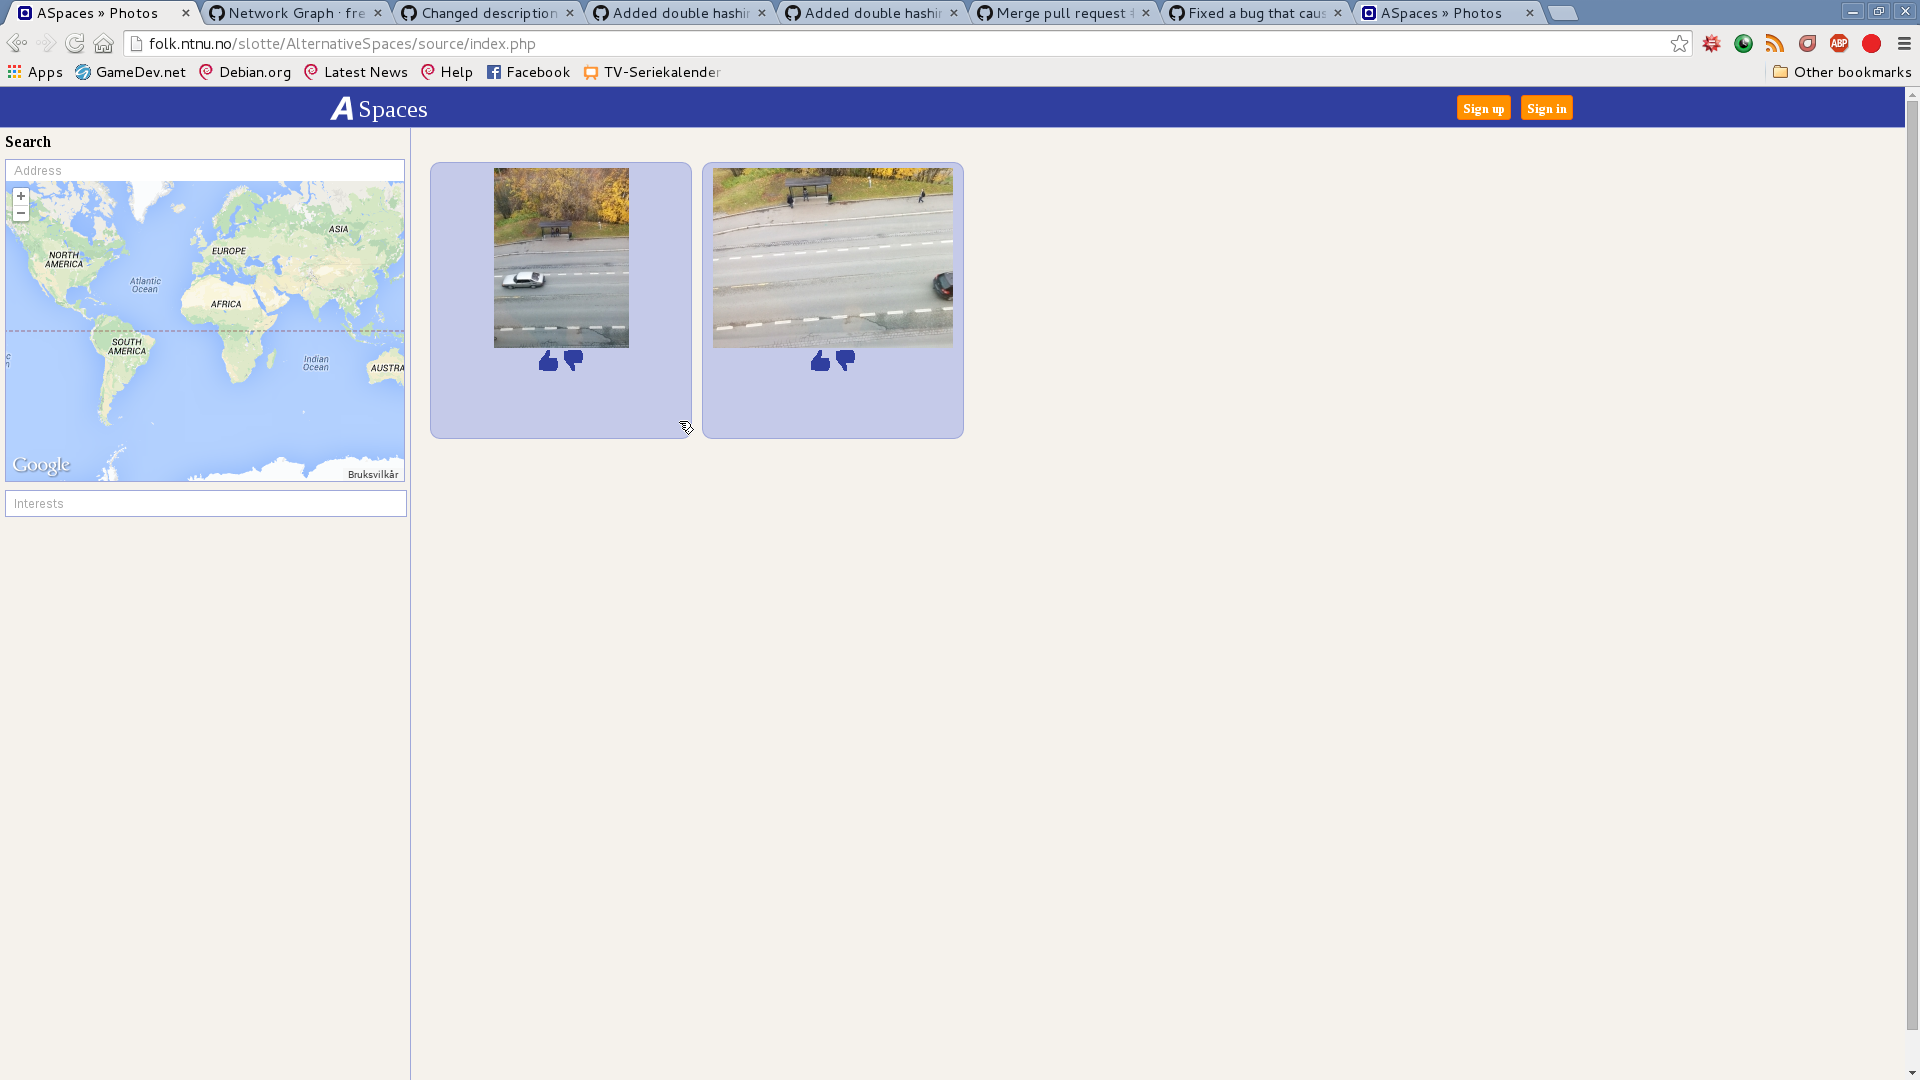
\includegraphics[width=\linewidth]{./img/webpage/27Oct/Frontpage27Oct}
  \caption{The first iteration of the new design for the front page.}
  \label{fig:S5DesignImplFront27Oct}
\end{figure}

\paragraph{} As mentioned in \ref{subsec:S2PresentationFeedback}, the most important problem with our site, after the lack of a mobile app, was the small size of the search map when in the photos view. As shown in figure \ref{fig:S5DesignImplFront27Oct}, we quadrupled the size of the map, which greatly increased the usability, and improved the use of space, especially on screens with high resolution.

\begin{figure}[ht!]
  \centering
  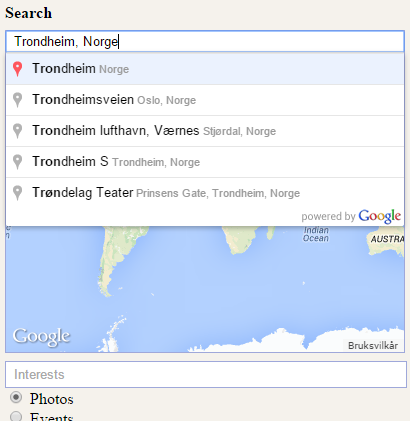
\includegraphics[width=70mm]{./img/webpage/27Oct/AddressAutocomplete.png}
  \caption{Address search with autocomplete feature.}
  \label{fig:S5DesignImplAddressAuto}
\end{figure}

\paragraph{} The next feature the youth had asked for was the ability to search for locations by address. We added this using the google maps API, including autocomplete for the address search, as shown in figure \ref{fig:S5DesignImplAddressAuto}.

\begin{figure}[ht!]
  \centering
  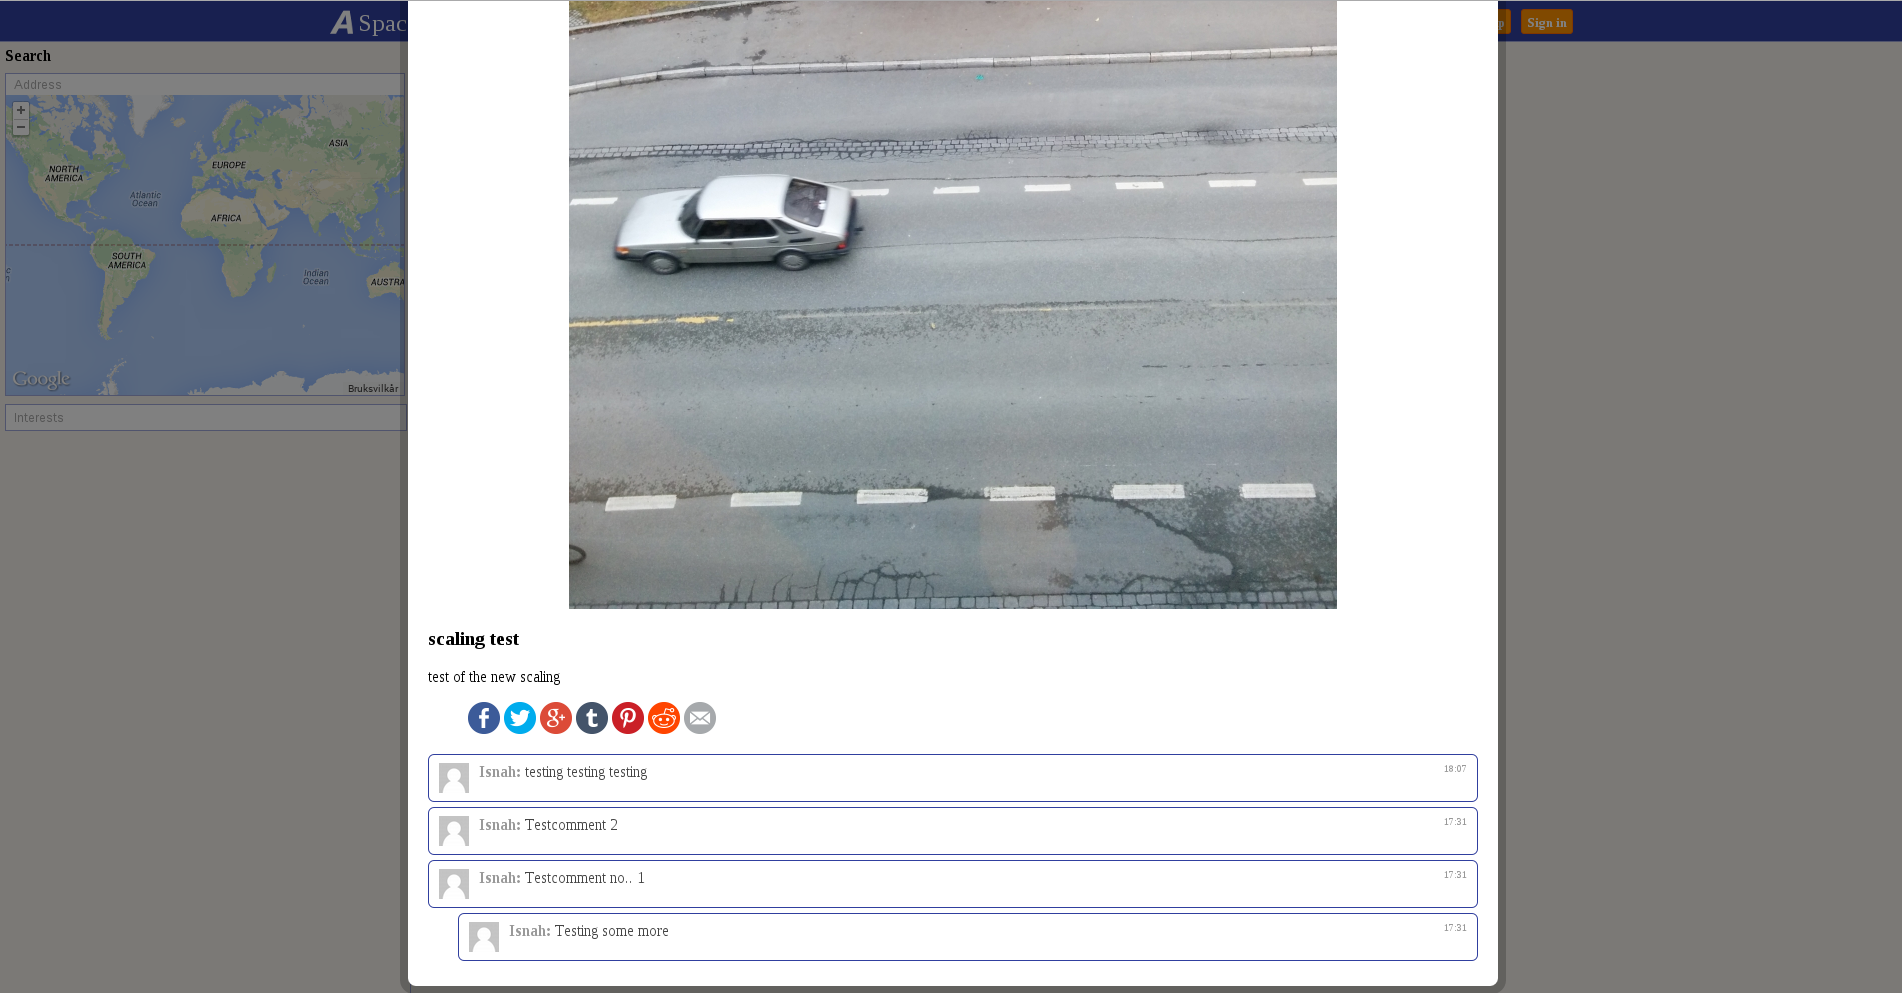
\includegraphics[width=\linewidth]{./img/webpage/27Oct/SinglePhoto27Oct}
  \caption{The photo overlay after the first week. The buttons for sharing the picture can be seen just below it.}
  \label{fig:S5DesignImplSinglePhoto27Oct}
\end{figure}

\paragraph{} Early on, we also added the ability to share pictures, and later on events, on other social media. This had been requested at the presentation, and it was fairly simple, and might add to the appeal of using the site. We considered it a good idea to have, as it might help expand the user base early on.

\paragraph{} Another thing to note is the new color scheme that was part of the new design. To find colors that worked well together, we looked through Google's design guidelines and tried several color combinations before landing on shades of indigo with an orange accent color.

\paragraph{} During the second part of the sprint, the design had been finalized, and we focused on geting the last few features we had decided to add into the prototype. The main part of the site was reduced to a single page with a choice of whether to view pictures or events. Voting on pictures and events was implemented to have a way of sorting them. The pictures were given a rating of 
\begin{equation} \label{eq:S5DesignImplSorting}
\frac{U-D}{|U-D|} Log_{10}(|U-D|) + \frac{t}{300000}
\end{equation}
where $U$ and $D$ are votes up and down, respectively, and $t$ is the UNIX timestamp at the time the picture is posted.
\subparagraph{} Events were simply given a rating based directly on the votes, since they are currently not shown on the page at all one day after the event is scheduled to happen.

\begin{figure}
\begin{minipage}{0.45\linewidth}
  \centering
  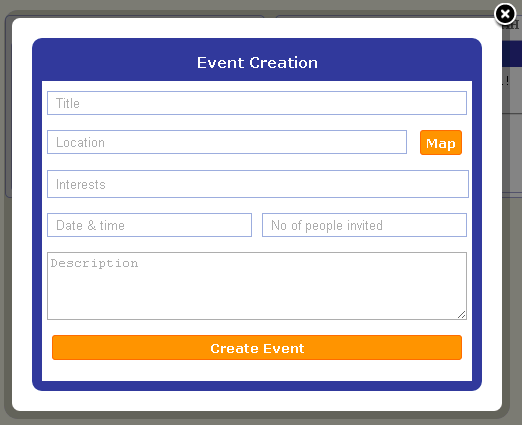
\includegraphics[width=\linewidth]{./img/webpage/3Nov/EventCreateBlank}
  \caption{The new event creation overlay.}
  \label{fig:S5DesignImplEventCreateBlank}
\end{minipage}%
\hspace{0.1\linewidth}
\begin{minipage}{0.45\linewidth}
  \centering
  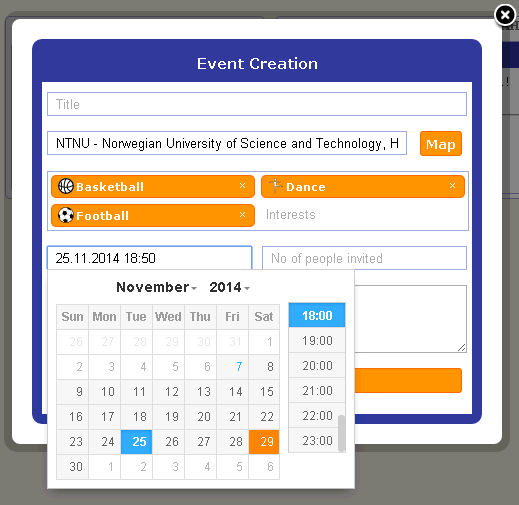
\includegraphics[width=\linewidth]{./img/webpage/3Nov/EventCreateCalendar}
  \caption{Choosing a date for an event using the calendar.}
  \label{fig:S5DesignImplEventCreateCalendar}
\end{minipage}
\end{figure}

\paragraph{} The event creation form was made. An empty form is shown in figure \ref{fig:S5DesignImplEventCreateBlank}, and a more filled in one in figure \ref{fig:S5DesignImplEventCreateCalendar}. It gives the ability to choose a location on a map, or writing the address, and choosing the time from a calendar. It also lets you specify the amount of people there is room for, but in the prototype this isn't used for anything beyond showing off the idea, since joining events has been pushed over to further work.

\begin{figure}[ht!]
  \centering
  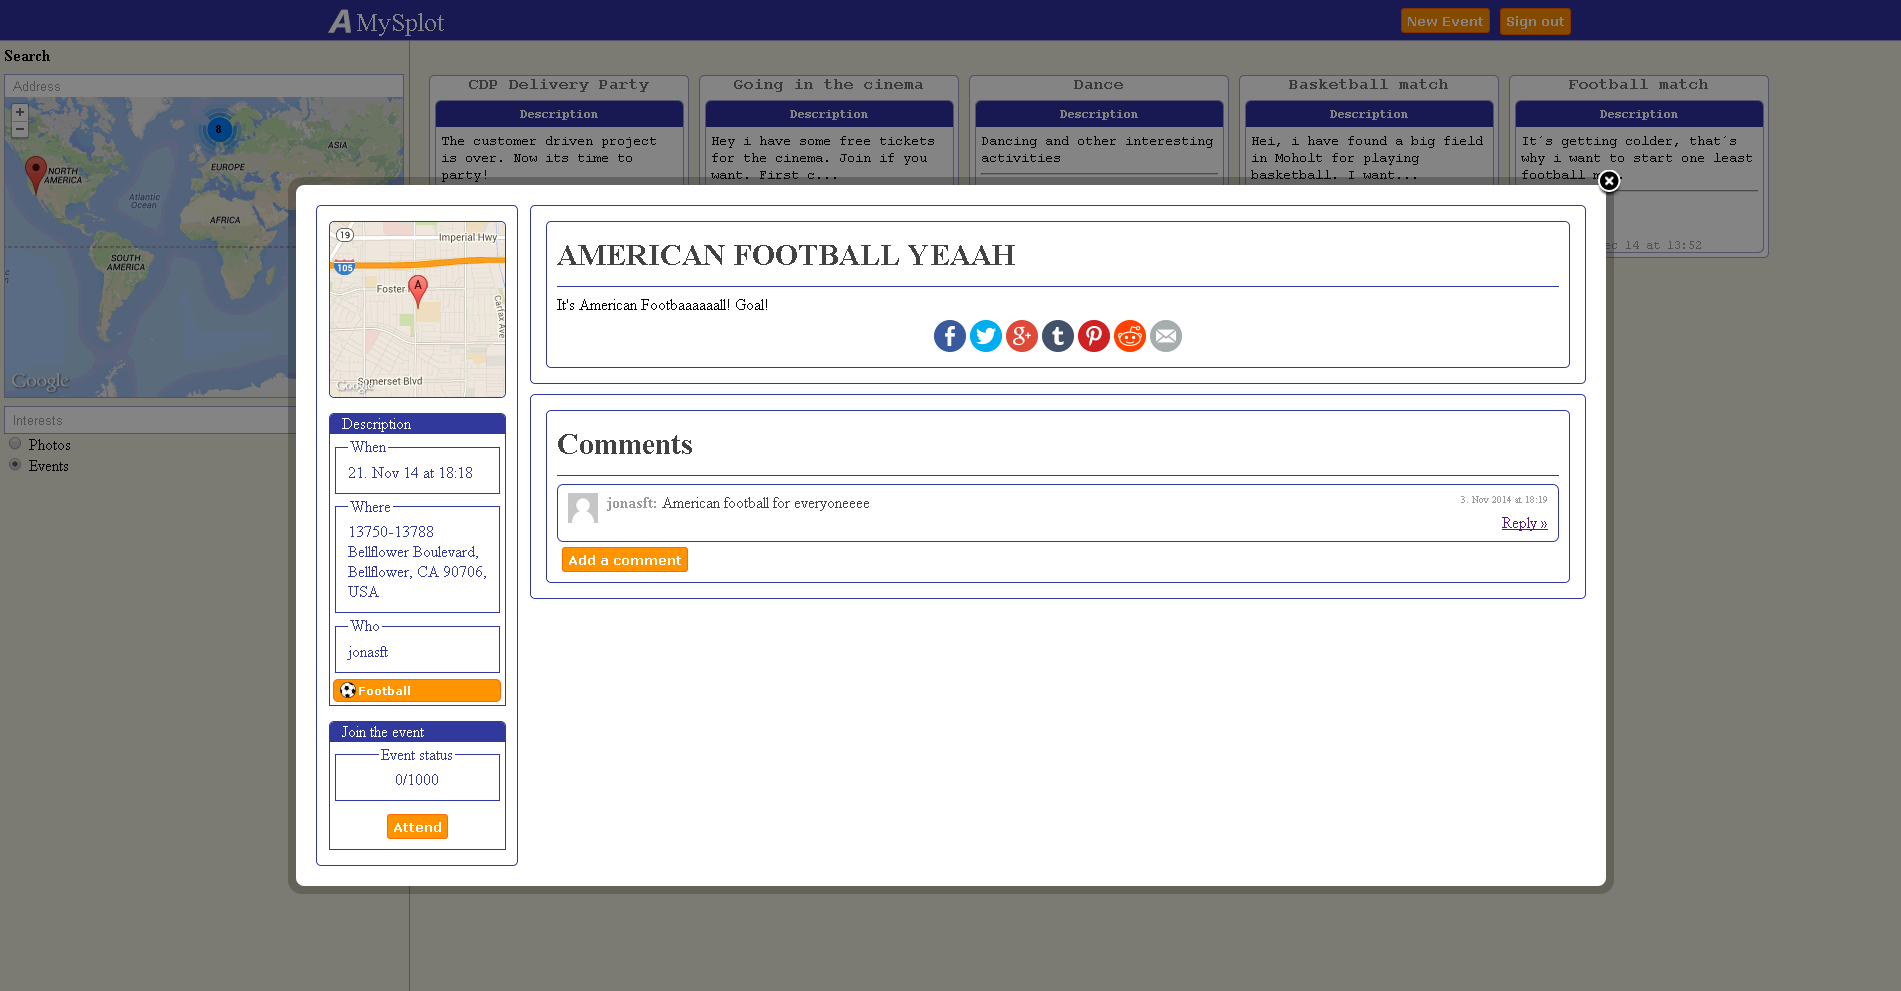
\includegraphics[width=\linewidth]{./img/webpage/3Nov/EventsOverlay}
  \caption{Overlay showing an event.}
  \label{fig:S5DesignImplEventsOverlay}
\end{figure}

\subparagraph{} The event page has been changed to an event overlay, to have a more consistent design by making events in the events page work the same way as photos on the photos page, as seen in figure \ref{fig:S5DesignImplEventsOverlay}. In the bottom left of the overlay, you can see the idea for events being limited by number of people, rather than having specific invites. The idea is discussed in \ref{chap:Further}

\begin{figure}[ht!]
  \centering
  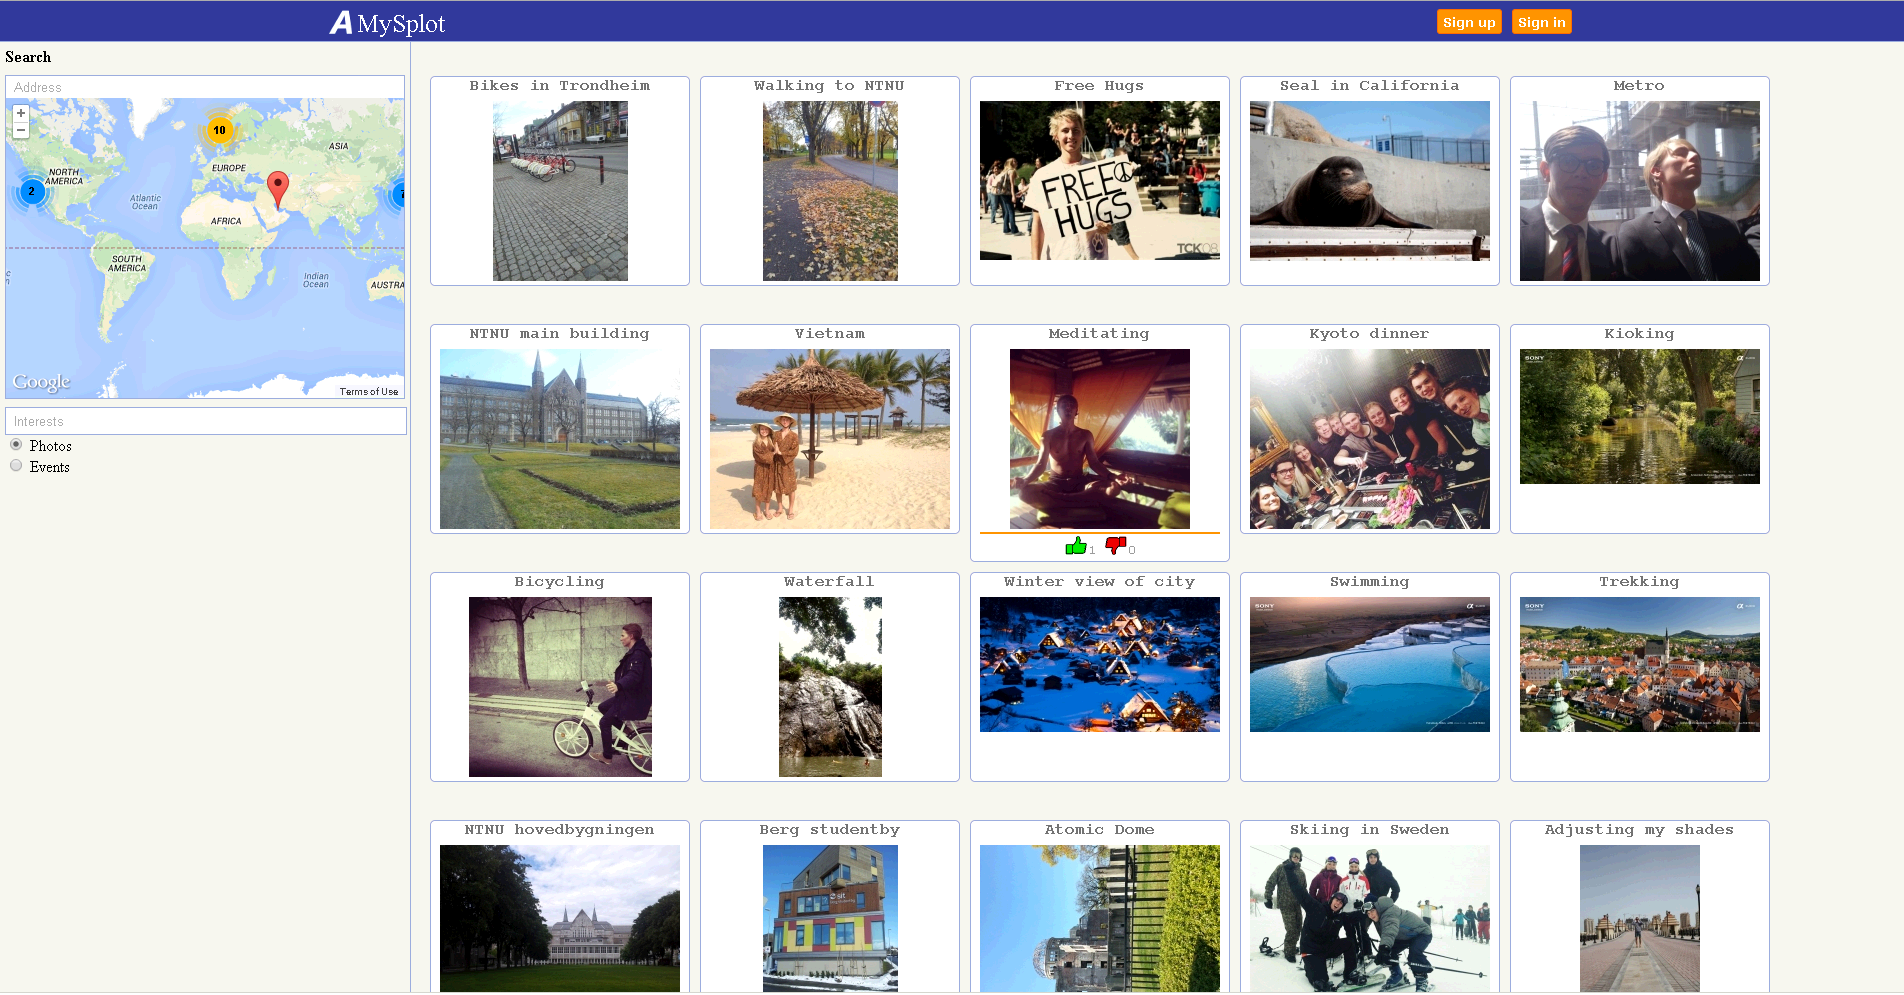
\includegraphics[width=\linewidth]{./img/webpage/3Nov/FrontpagePhotos}
  \caption{The design of the front page at the end of the sprint.}
  \label{fig:S5DesignImplFrontPhotos3Nov}
\end{figure}

\paragraph{} As mentioned earlier in this sections, voting was implemented for both photos and events. There were also other improvements to the photos page, both for the whole page and the single photo overlay. As seen in \ref{fig:S5DesignImplFrontPhotos3Nov}, the vote buttons got their final design, and just below the map you can choose whether you want to see photos or events. This design for the choice of view was made with expandability in mind. It should be simple to use this design to add other views, such as a video page or a free comment page.

\begin{figure}[ht!]
  \centering
  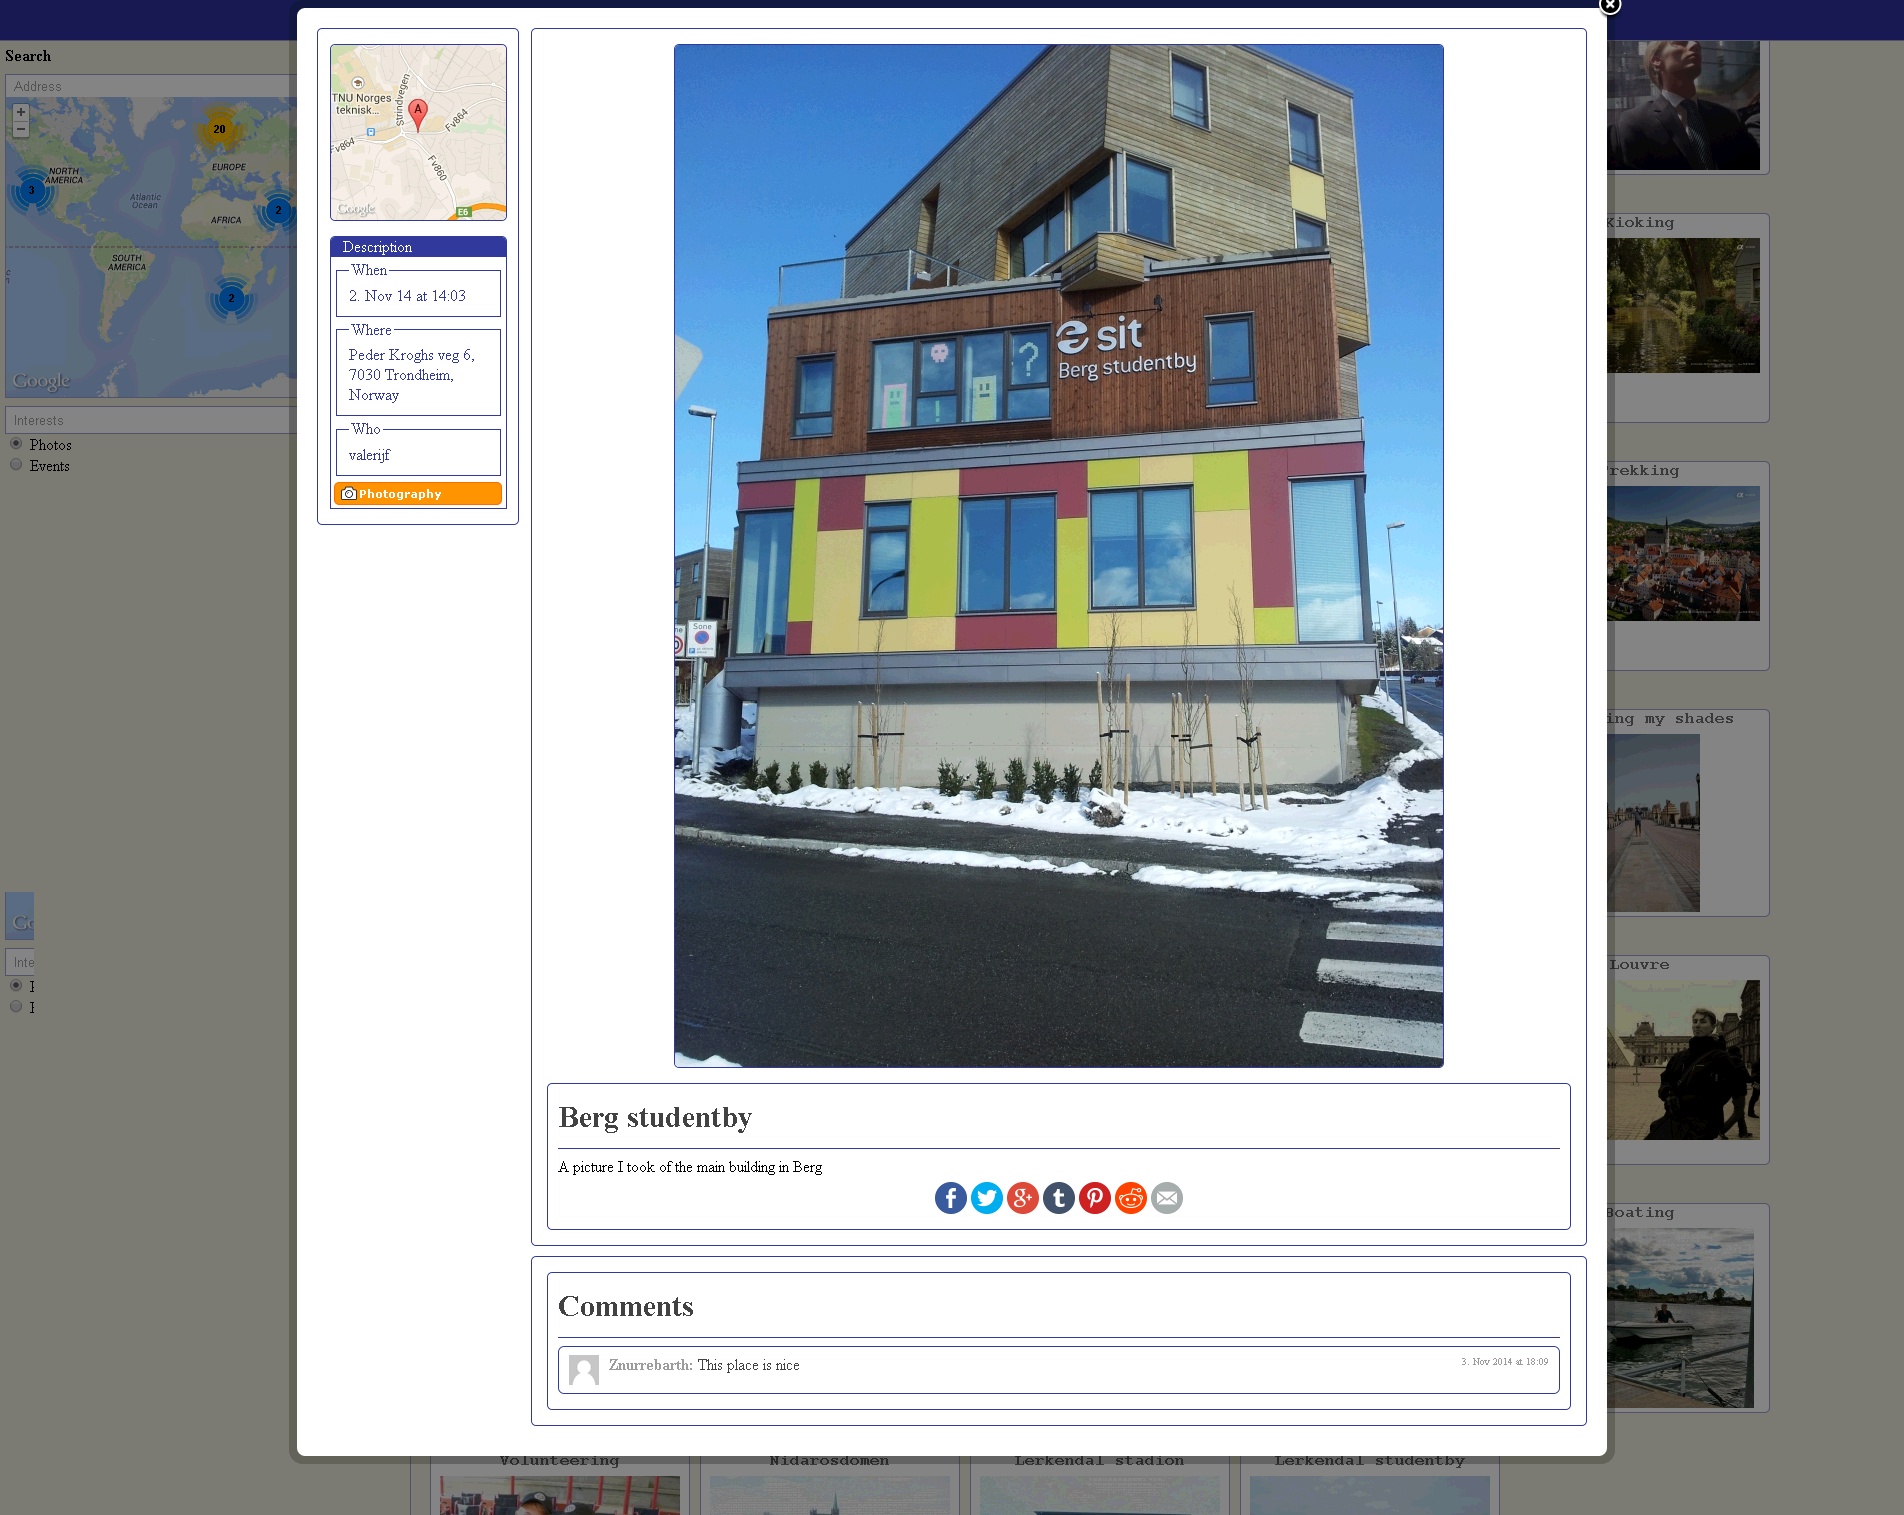
\includegraphics[width=\linewidth]{./img/webpage/3Nov/PhotoOverlay}
  \caption{The single photo overlay at the end of sprint 4.}
  \label{fig:S5DesignImplPhotoOverlay3Nov}
\end{figure}

\paragraph{} The end users had requested that the pictures should have more information displayed, as seen in figure \ref{fig:S5DesignImplPhotoOverlay3Nov}, we implemented the overlay to now show location, user, and upload time, as well as the interests a picture has been tagged with. If you look close at the interest tag, you'll also note that the interests now have a small logo added to them. This is for quick identification in the events page, where only the icon is shown unless the mouse pointer hovers over the it.

\begin{figure}[ht!]
  \centering
  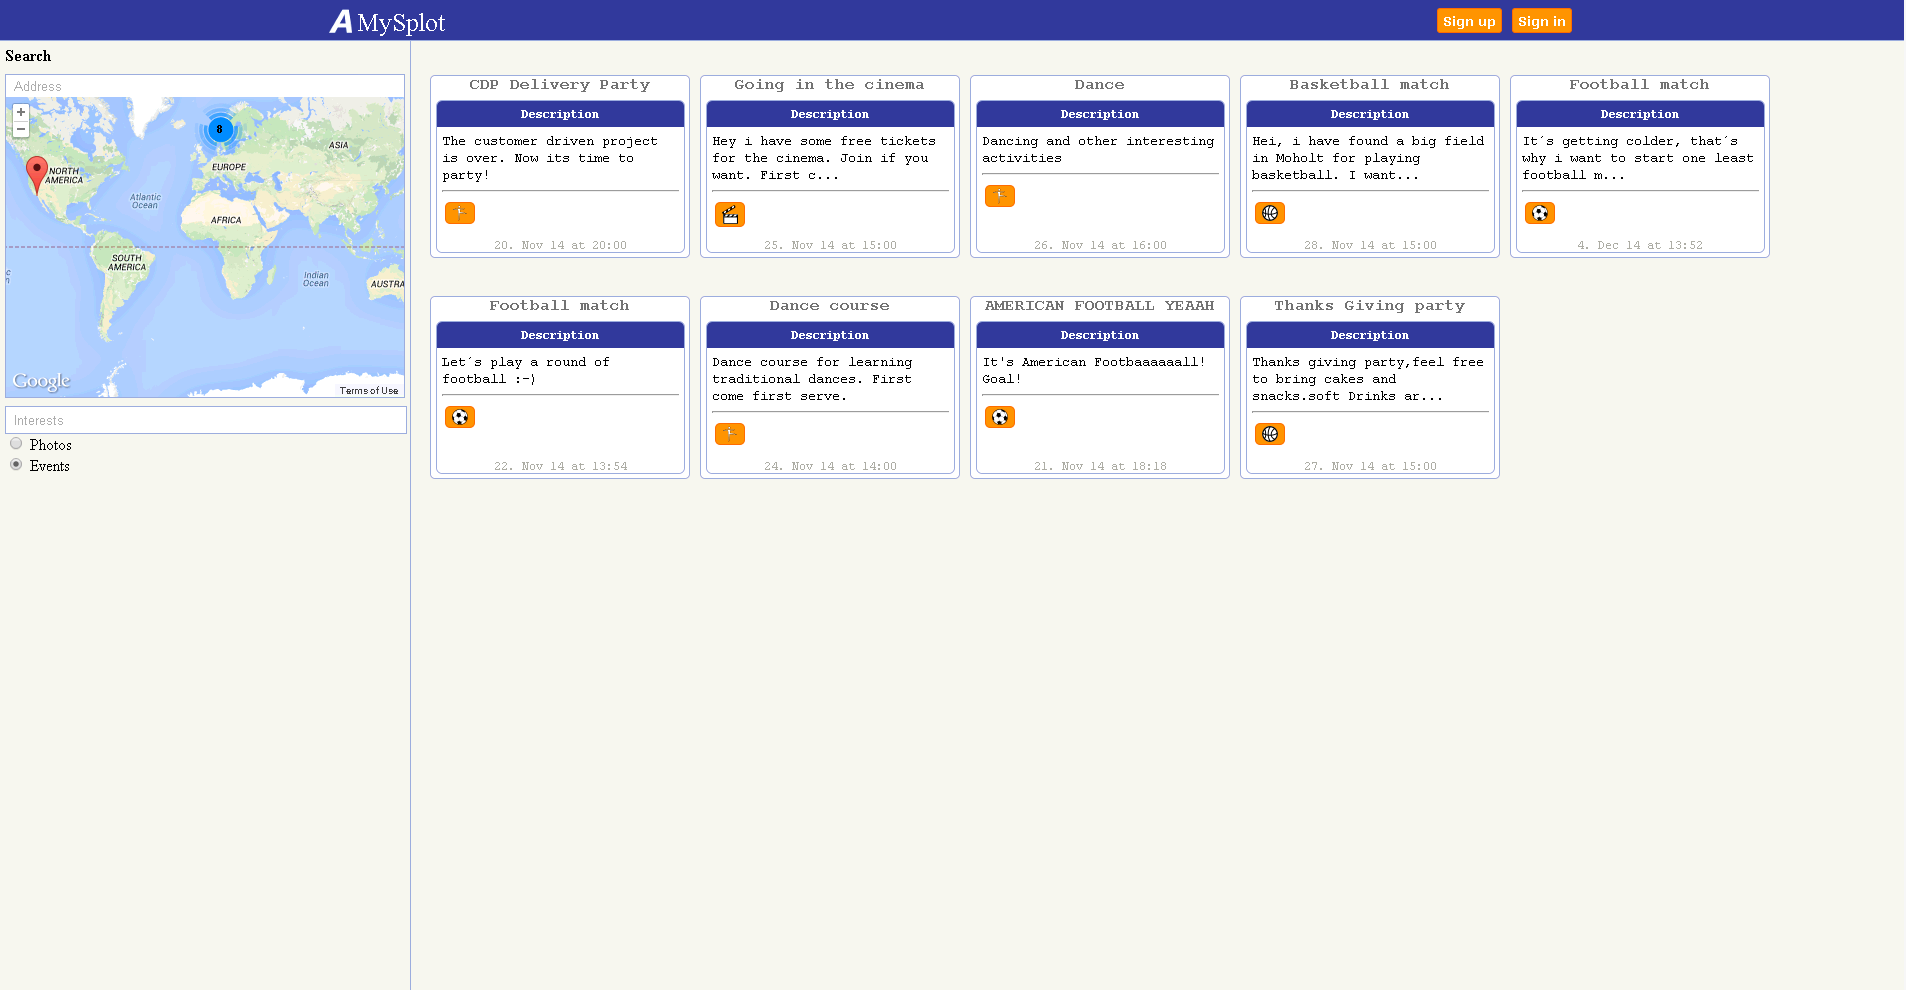
\includegraphics[width=\linewidth]{./img/webpage/3Nov/FrontpageEvents}
  \caption{The event page at the end of sprint 4.}
  \label{fig:S5DesignImplFrontEvents3Nov}
\end{figure}

\begin{figure}[ht!]
  \centering
  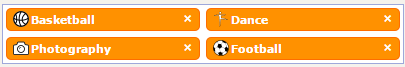
\includegraphics[width=80mm]{./Sprint5/img/InterestIcons}
  \caption{Interests with icons.}
  \label{fig:S5DesignImplInterestIcons}
\end{figure}

\paragraph{} As mentioned in section \ref{sec:S5Plan}, the Technical Lead spent some time helpping the customers get a domain for the website, and the site up on that domain. At the beginning of the sprint, we spent some time trying to come up with good domain names, and we sent some suggestions to the customer. In the end, they chose on their own, and landed on the name mysplot.com, with splot being a conflation of spot and lot. The customer then told us they'd get a hold of some art for icons etc, which we would use in the final part to finish the look of the site.


\section{Testing and Results}
\label{sec:S5Testing}
\paragraph{} During this sprint, testing was done during the Design and implementation phase, and the functionality of the code actively tested on the go. Before the new functionality was merged into the master branch, all new functionality had been tested and ensured working. 

\paragraph{} All the features of mysplot.com for this sprint were functionally tested, as explained in the first part of the report. For example the social media sharing posts have been tested by clicking the sharing icons available on the event overlay page, then sharing the media to the corresponding network cliked. See below. 

\paragraph{} The final results of the fourth sprint include completing all the sprint backlog items. Based on the feedback from the presentation. The design of the 2D search was updated, mainly increasing the size of the map and adding the possibility of searching adresses in the search bar. This makes the map more usable, with more precise navigation and greater view. The search bar giving the users a new possibility of limiting the map to an area of their choice by inputing a location in the search bar. Next, the media posts now have a rating function to calculate relevance, the event form reached its final version, and theme colors of the webpage were updated to indigo and orange. Finally, the design of the individual photo and event pages were completed, now as more detailed overlay windows. As the sprint was came close to and end, the entire product was installed on “www.mysplot.com”. 

%%%%%%%%
%FIGURES
%%%%%%%%

\begin{figure}[ht!]
  \centering
  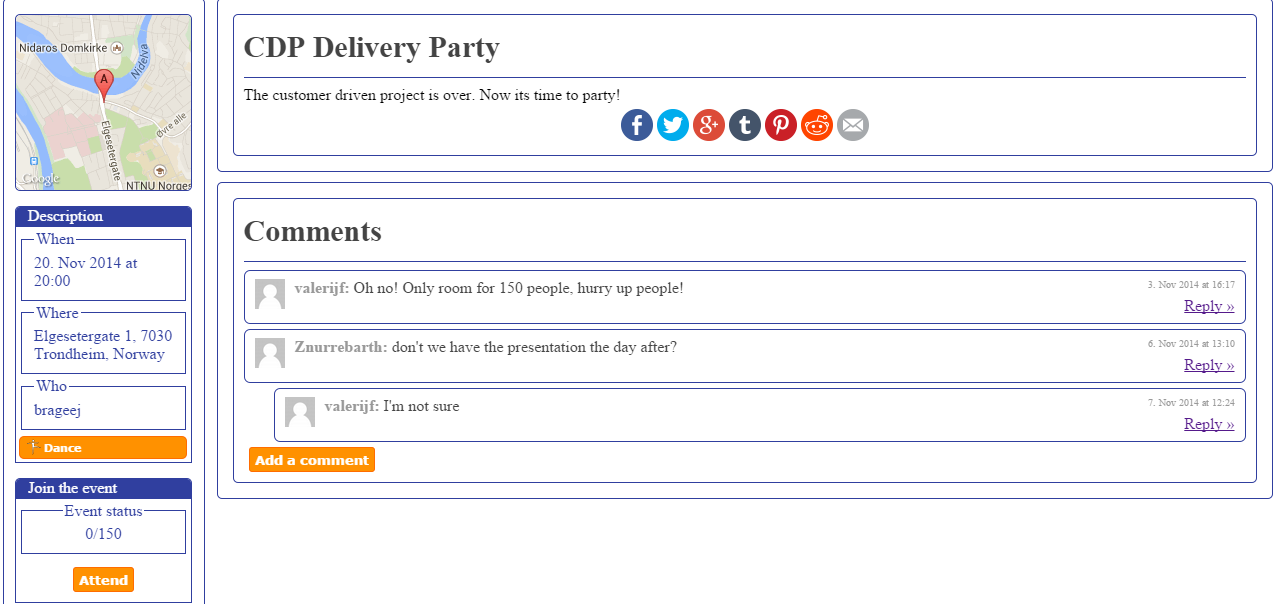
\includegraphics[width=\linewidth]{Sprint5/img/test1.png}
  \caption{The event page, with the clickable icons below the event's description with the functionality of sharing the event to other social networks. }
  \label{fig:S5TestMediaIconClick}
\end{figure}

\begin{figure}[ht!]
  \centering
  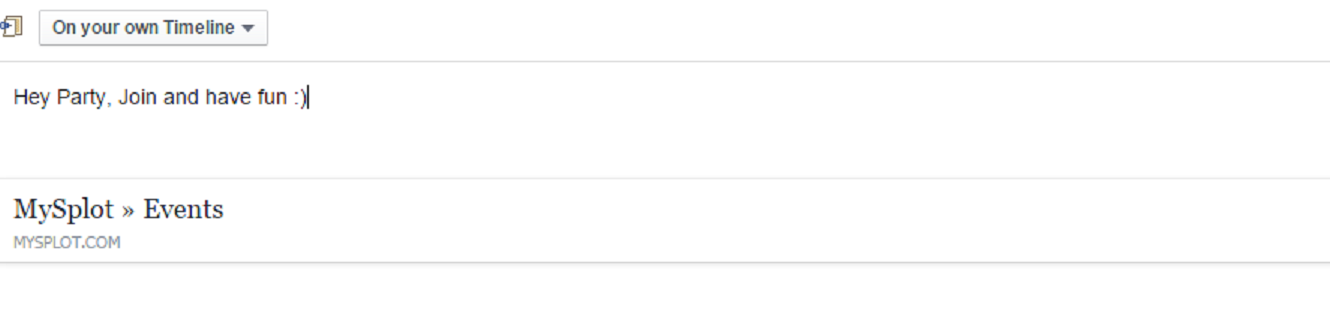
\includegraphics[width=50mm]{Sprint5/img/test2.png}
  
\includegraphics[width=50mm]{Sprint5/img/test3.png}
  \caption{Views during the process of sharing a mysplot-event onto the social network ``Facebook''. }
  \label{fig:S5TestSharingFacebook}
\end{figure}

\begin{figure}[ht!]
  \centering
  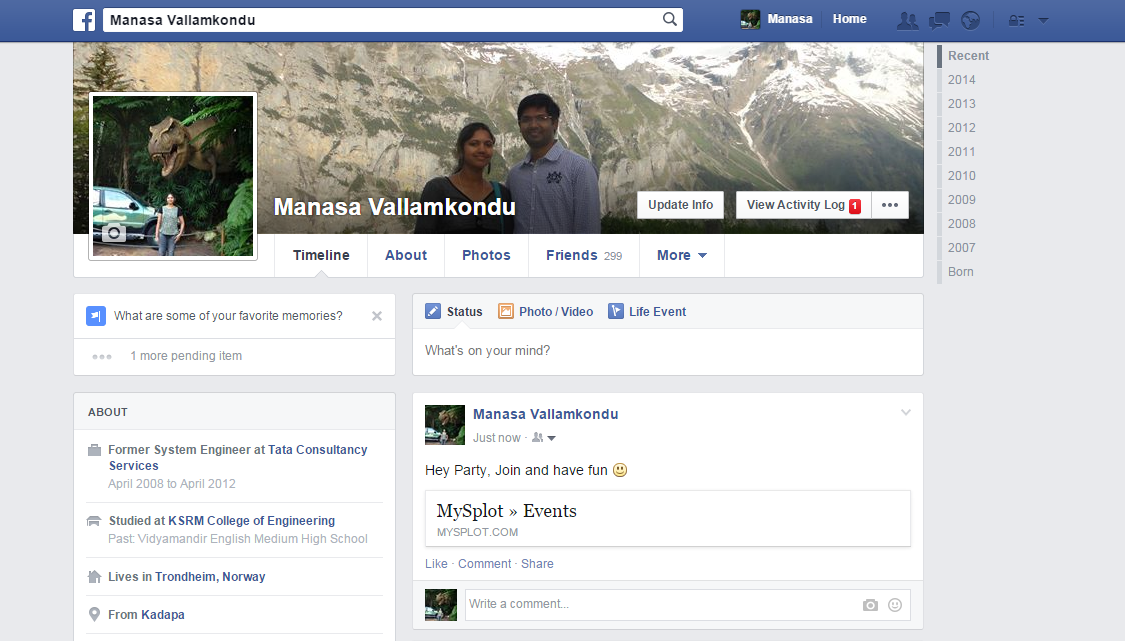
\includegraphics[width=\linewidth]{Sprint5/img/test4.png}
  \caption{Final view of an event posted to Facebook.}
  \label{fig:S5TestFacebookView}
\end{figure}

\begin{figure}[ht!]
  \centering
  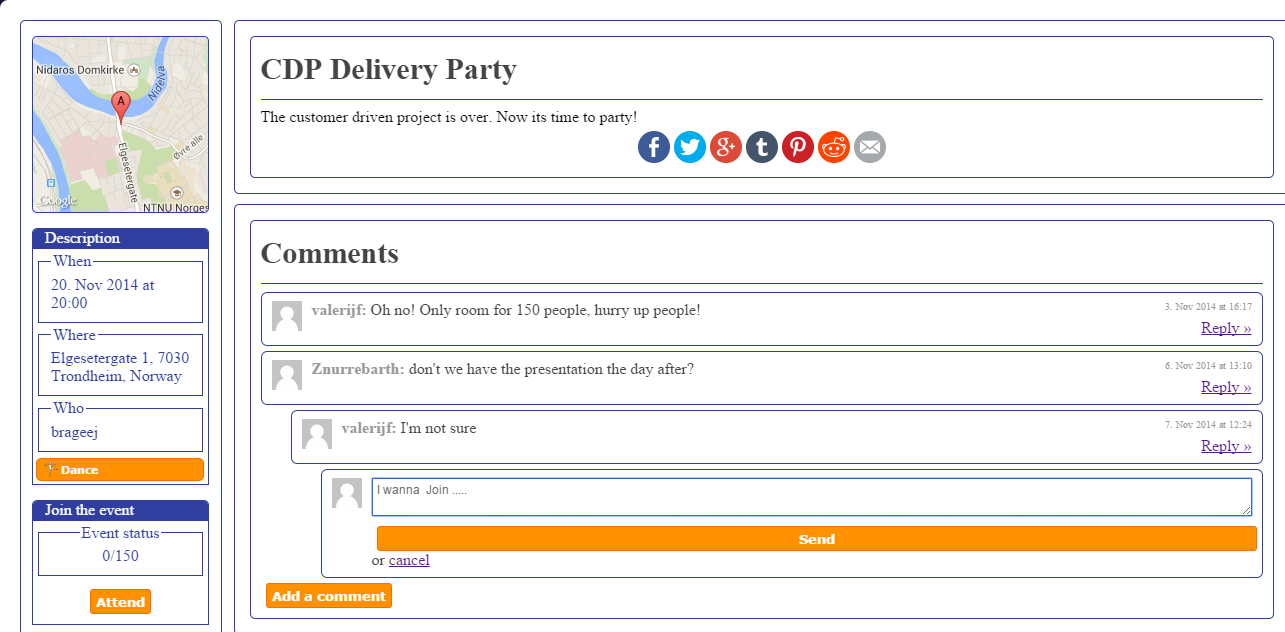
\includegraphics[width=90mm]{Sprint5/img/test5.png}
  \caption{View while commenting on an event, before clicking the ``Reply button''. }
  \label{fig:S5TestBeforeComment}
\end{figure}

\begin{figure}[ht!]
  \centering
  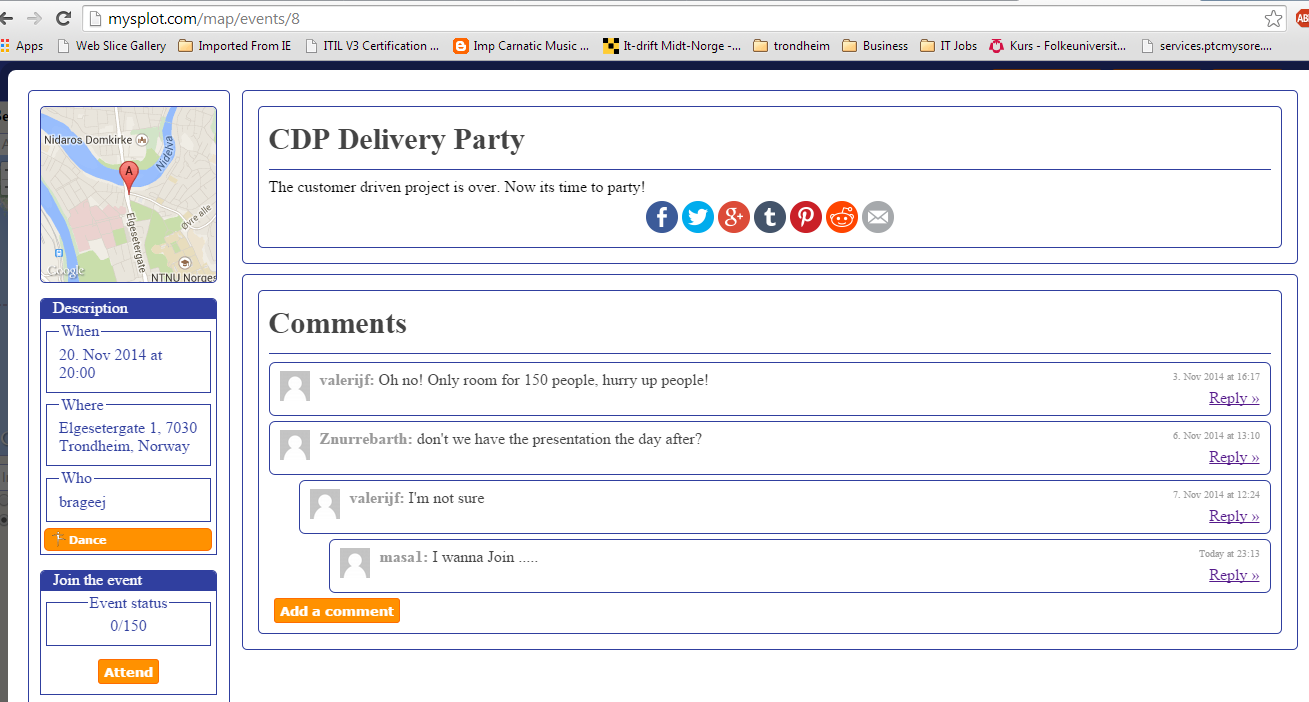
\includegraphics[width=90mm]{Sprint5/img/test6.png}
  \caption{View after commenting on an event. }
  \label{fig:S5TestAfterComment}
\end{figure}

\begin{figure}[ht!]
  \centering
  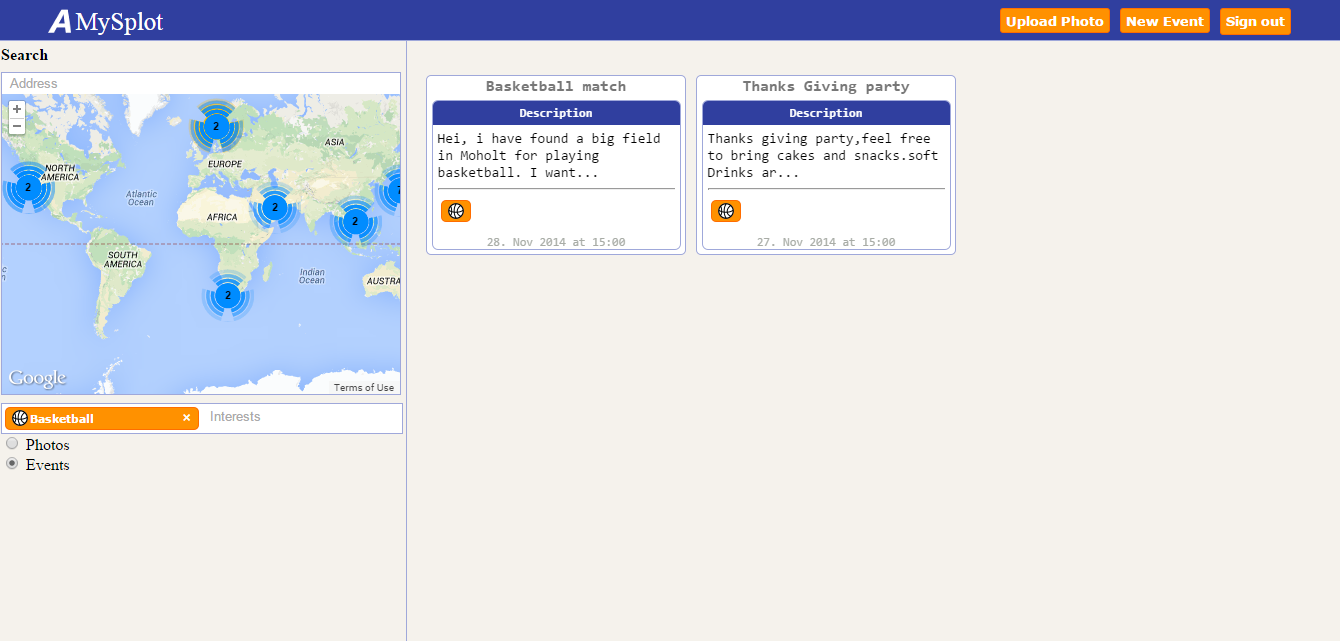
\includegraphics[width=\linewidth]{Sprint5/img/test7.png}
  \caption{View of the homepage when searching for events tagged with the interest ``Basketball''. }
  \label{fig:S5TestAfterComment}
\end{figure}

\newpage
\section{Sprint retrospective}
\label{sec:S5Retrospective}



\subsection{Start doing}
\label{subsec:S5RetrospectiveStart}

\begin{itemize}
  \item Test the web application thoroughly.
  \item The report work should be uploaded in Google docs immediately after completion so they can be proof read by other group members.
  \item Update the work sheet after every work session. Each time people forget, the error of estimation increases. 
  \item Explore ways of improving your writing skills. 
\end{itemize}

\subsection{Stop doing}
\label{subsec:S5RetrospectiveStop}
\begin{itemize}
\item Showing up late to meetings. 
\end{itemize}

\subsection{Continue doing}
\label{subsec:S5RetrospectiveContinue}

\begin{itemize}
  \item Work in group for discussing report sections.
  \item Perfecting the product by debugging. 
\end{itemize}

\subsection{Group dynamics}
\label{subsec:S5RetrospectiveDynamics}

Compared to the previous 
Still the number of hours per person has to be increased by 20\% to 30\% according to compendium. But for sprint 5, we have 70\% of the total hours (20 hrs per person).
In the sprint 5, few of the group members were away and couldn’t contribute more work hours, the report assignments were bit slow, but the system is completely developed with all the agreed changes suggested by the user and customer. The domain has been set up and the whole group tested the various functionalities of the Application and bugs were raised accordingly. Part of the group was working for the Bug fixing, the rest of the group in writing the report and implementing all the report work into Latex.

